\documentclass[line,margin]{res} 
\hyphenation{de-sa-rro-llo man-te-ni-mien-to}
%\usepackage{helvetica} % uses helvetica postscript font (download helvetica.sty)
%\usepackage{newcent}   % uses new century schoolbook postscript font 

\usepackage{simplemargins}
\setleftmargin{0.5in}
\setrightmargin{2.0in}
\settopmargin{0.7in}
\setbottommargin{0.3in}


\usepackage{hyperref}
%\hyperref[mainlemma]{lemma \ref{mainlemma}}
\hypersetup{
    bookmarks=false,         % show bookmarks bar?
    unicode=false,          % non-Latin characters in Acrobats bookmarks
    pdftoolbar=false,        % show Acrobats toolbar?
    pdfmenubar=true,        % show Acrobats menu?
    pdffitwindow=true,     % window fit to page when opened
    pdfnewwindow=true,      % links in new window
    colorlinks=true,       % false: boxed links; true: colored links
    linkcolor=red,          % color of internal links
    citecolor=green,        % color of links to bibliography
    filecolor=magenta,      % color of file links
    urlcolor=blue           % color of external links
}

\usepackage{graphicx} 

%\addtolength{\oddsidemargin}{-0.875in}
%\addtolength{\evensidemargin}{-0.875in}
%\addtolength{\textwidth}{1.5in}
%
%\addtolength{\topmargin}{-0.875in}
%\addtolength{\textheight}{1.5in}


\begin{document}

\name{Roberto Arias Ruiz}
% \address used twice to have two lines of address
%\address{Calle Laforja, 8. pral-1era, 08006. Barcelona, Espa\~{n}a}
\address{+34 678714822 / roberlamerma@gmail.com}

\begin{resume}
 
\section{PERFIL PERSONAL}       
                \begin{itemize}  \itemsep 2pt % reduce space between items
                \item  Ingeniero Inform\'{a}tico Superior con amplia 
                experiencia en an\'{a}lisis, dise\~{n}o, desarrollo y 
                mantenimiento de software en diversas plataformas, sistemas 
                operativos.
                \item Amplia experiencia en gesti\'{o}n de proyectos y grupos de 
                trabajo, especialmente con equipos que se rigen por metodolog\'{i}a \textit{SCRUM}.
                \item Capacidad de an\'{a}lisis y resoluci\'{o}n de problemas en 
                tiempo cr\'{i}tico y/o bajo presi\'{o}n.
                \item Excelente capacidad de comunicaci\'{o}n y articulaci\'{o}n 
                (Ingl\'{e}s y Castellano).
%                \item{\hskip-.25in\llap{1997}\hskip.25in{}worked here} 
%                \item{\hskip-.25in\llap{\parbox[b]{1in}{This is a longer note that might wrap}}\hskip.25in{}worked there}
                \end{itemize}
         

\section{EXPERIENCIA \\LABORAL \\ \footnotesize{(referencias disponibles)}}

{\sl Software Configuration Manager} \hfill Mayo 2011 -- Ahora \\
                \textbf{Roche Diagnostics} 
                $<$\url{http://www.roche.com/diagnostics/}$>$ \hfill \textit{Sant Cugat, Espa\~{n}a}
                \begin{itemize}  \itemsep 2pt % reduce space between items
                \item Responsable de definici\'{o}n y administraci\'{o}n de \textit{Builds} en TFS.
                \item Definici\'{o}n de estrategia de \textit{Branching and Merging} entre 4 equipos,
                distribuidos en sedes diferentes (Sant Cugat y Rotkreuz, Suiza). Metodolog\'{i}a SCRUM
                \item An\'{a}lisis funcional y de requerimientos. Sincronizaci\'{o}n automatizada de tests desde VS2010 
                a HPQC \textit{(HP Quality Center)}, para garantizar cobertura de requerimientos.
                \item Arquitectura de aplicaciones: EA \textit{(Enterprise Architect}) y HPQC.
                \end{itemize}


				{\sl Arquitecto} \hfill Abril 2010 -- Mayo 2011 \\
                \textbf{Wolters Kluwer} 
                $<$\url{www.wolterskluwer.es}$>$ \hfill \textit{Barcelona, Espa\~{n}a}
                \begin{itemize}  \itemsep 2pt % reduce space between items
                \item An\'{a}lisis funcional y T\'{e}cnico de un \textit{Framework} de desarrollo 
                para un proyecto conjunto entre las sedes Europeas de la empresa.
                \item Desarrollo de componentes \textit{CORE} del framework: Librer\'{i}a \textit{custom}
                de controles WPF; arquitectura centralizada para comunicaciones WCF y Silverlight.
                \item Cordinaci\'{o}n con equipo de desarrollo \textit{(outsourcing partners)} 
                de la India. Rol: \textit{Scrum Master}.
                \item .Net 4.0, C{\#}, SQL Server, WCF, WPF, Silverlight. DDD \textit{Domain Driven Design}
                \\
                \end{itemize}
                
                {\sl Analista Programador} \hfill            Marzo 2007 -- Febrero 2010 \\
                \textbf{Knosos, Grupo Amper} 
                $<$\url{www.amper.es}$>$ \hfill \textit{Barcelona, Espa\~{n}a}
                \begin{itemize}  \itemsep 2pt % reduce space between items
                \item Licitaci\'{o}n de proyectos (documentaci\'{o}n) 
                seg\'{u}n normativa IEEE/EIA 12207 e ISO 9001.
                \item Ingenier\'{i}a de software: Requerimientos, an\'{a}lisis y 
                dise\~{n}o (UML), estimaci\'{o}n de recursos, desarrollo, 
                pruebas (Test Units, Benchmarking, Profiling) y mantenimiento. 
                Control de versiones y despligues de software.
                \item Estrategias, dise\~{n}o e implementaci\'{o}n de servicios 
                utilizando el marco ITIL.
                \item Dise\~{n}o de servicios y aplicaciones .NET: modelos 
                Cliente-Servidor, MVC y aplicaciones distribuidas de alta 
                disponibilidad. Tecnolog\'{i}as: WPF, WCF, Remoting, SOAP, 
                Compact Framework, Sockets, etc.
                \item Investigaci\'{o}n y desarrollo de sistemas embebidos y 
                aplicaciones m\'{o}viles.
                \\
                \end{itemize}


                {\sl Analista Programador} \hfill Diciembre 2005 -- Enero 2007 \\
                \textbf{Grupo 3C} 
                $<$\url{www.tresce.com}$>$ \hfill \textit{Barcelona, 
                Espa\~{n}a}
                \begin{itemize}  \itemsep 2pt % reduce space between items
                \item Tuning de Apache e IIS. Manejo de entornos de 
                alta disponibilidad, redundados.
                \item Desarrollo de sistemas Web: PHP, Perl. Tecnologas: HTML, 
                CSS y Javascript. AJAX.
                \item T\'{e}cnicas SEO. Indexaci\'{o}n y PageRank. Manejo de 
                herramientas de an\'{a}lisis Web e indexaci\'{o}n: 
                Google Analytics, Google Sitemaps, Google API, etc.
                \\
                \end{itemize} 

                {\sl Programador Freelance} \hfill Agosto 2004 -- Octubre 
                2005 \\
                \textbf{iChameleon Group INC} 
                $<$\url{www.ichameleongroup.com}$>$ \hfill \textit{Miami, EEUU}
                \begin{itemize}  \itemsep 2pt % reduce space between items
                \item Proyecto freelance, para desarrollar la plataforma 
                (Frontend y Backend) de una tienda de m\'{u}sica online. Perl, 
                FastCGI, PostgreSQL.
                \item Desarrollo de aplicaciones cliente para Mac (Apple), en el 
                lenguaje Objective-C, bajo el Framework Cocoa.
                \\
                \end{itemize}

                {\sl Programador (pr\'{a}cticas)} \hfill Agosto 2003 -- Julio 
                2004 \\
                \textbf{Gaiax Co, LTD} 
                $<$\url{www.gaiax.co.jp}$>$ \hfill \textit{Tokio, 
                Jap\'{o}n}
                \begin{itemize}  \itemsep 2pt % reduce space between items
                \item Dise\~{n}o y desarrollo de un portal de juegos para 
                japoneses, utilizando Perl (mod\_perl y FastCGI)
                \\
                \end{itemize} 

                {\sl Administrador de Sistemas} \hfill Octubre 1999 -- Julio 
                2002 \\
                \textbf{Laboratorio de Computaci\'{o}n, USB} 
                $<$\url{www.ldc.usb.ve}$>$
                \hfill \textit{Caracas, Venezuela}
                \begin{itemize}  \itemsep 2pt % reduce space between items
                \item Dise\~{n}o y mantenimiento de varios nodos de la LAN 
                universitaria. Mantenimiento de todo el software: NFS, Samba, LDAP, Mail, etc.
                \item Red 100\% Unix, con servidores \textit{Linux} y \textit{Solaris}.
                \end{itemize}

\section{LOGROS}       
                \begin{itemize}  \itemsep 2pt % reduce space between items
                \item Implementaci\'{o}n exitosa (Wolters Kluwer) de estrategia de colaboraci\'{o}n 
                con 3 equipos de desarrollo diferentes, localizados en India. Liderazgo de uno de dichos equipos.
                \item Coordinaci\'{o}n del equipo que en conjunto con 
                EUROCONTROL (\url{www.eurocontrol.int}), dise\~{n}\'{o} e 
                implement\'{o} el protocolo de datos ASTERIX, utilizado en 
                diversas soluciones de Amper en el \'{a}mbito militar a nivel 
                Espa\~{n}ol y Europeo.
                \item Dise\~{n}o e implementaci\'{o}n de un protocolo de 
                transporte y transmisi\'{o}n de paquetes de datos a trav\'{e}s 
                de la red SIRDEE (Tetrapol)
                \item Puesta en marcha de la plataforma (Jira + Confluence. 
                \url{www.atlassian.com}) que implementa la nueva metodolog\'{i}a 
                de gesti\'{o}n de tareas y gesti\'{o}n documental utilizada por 
                Knosos/Amper.
                \item Dise\~{n}o, puesta en marcha y mantenimiento de servidores 
                y servicios de Red en mltiples plataformas de comunicaciones: 
                GPRS, Tetra, TETRAPOL, Inmarsat, para Knosos/Amper.
                \item Coordinaci\'{o}n del proyecto (3C Formaci\'{o}n) para la 
                automatizaci\'{o}n de todos los procesos de an\'{a}lisis de 
                informaci\'{o}n en tiempo real.
                \item Mejora del posicionamiento (SEO) e indexaci\'{o}n (Google) 
                de varios portales web (3C Formaci\'{o}n).
                \item Desarrollo e implementaci\'{o}n (Gaiax, Co, LTD) de un 
                juego masivo en l\'{i}nea (\url{sugolog.cafe.ocn.ne.jp}), el 
                cual actualmente mantiene una popularidad importante en el 
                mercado japon\'{e}s.
                \item Como Administrador de Sistemas en el LDC, fui parte del 
                equipo que dise\~{n}\'{o} la nueva topolog\'{i}a de la LAN 
                universitaria, adem\'{a}s de la puesta a punto de todos los 
                servicios de red.
                \item Fui el responsable estudiantil del laboratorio (disponibilidad, 
                procesos de admisi\'{o}n, etc) durante mis \'{u}ltimos dos a\~{n}os en 
                la universidad. 
                \end{itemize}

\section{EDUCACI\'{O}N}
               \textbf{M\'{a}ster en Seguridad de las Tecnolog\'{i}as de la 
               Informaci\'{o}n,} \hfill Octubre 2006  Agosto 2007 \\
               \textit{Fundaci\'{o}n la Salle / Universitat Ram\'{o}n Llull} 
               \hfill Barcelona, Espa\~{n}a

               \textbf{Ingenier\'{i}a superior Inform\'{a}tica,} \hfill 
               Septiembre 1997 -- Julio 2003 \\
               \textit{Universidad Sim\'{o}n Bol\'{i}var} \hfill Caracas, 
               Venezuela

%               \textbf{Primaria - Bachillerato,} \hfill Octubre 1985 -- Julio 
%               1997 \\
%               \textit{Colegio San Ignacio de Loyola} \hfill Caracas, Venezuela


 
\section{CURSOS}
               \begin{itemize}  \itemsep 2pt % reduce space between items
               \item \textbf{CCNA} de Cisco (dise\~{n}o de redes, routing  y 
               switching)
               \item Certificado \textbf{ITIL} Foundations v3 (management, 
               desarrollo, operaciones y servicios en IT)
               \item \textbf{OPST} de ISECOM (an\'{a}lisis y testing de 
               seguridad)
               \item Curso avanzado en tecnolog\'{i}as \textbf{VMWare} 
               (virtualizaci\'{o}n)
               \end{itemize}


\section{IDIOMAS} 
               %\hfill 1: B\'{a}sico, 2: Regular, 3: Intermedio, 4: Experto, 
               %5: Materno \\ \\
               \textbf{Ingl\'{e}s,}
               nivel conversacional, escrito y leido: \textit{avanzado}.
               \\
               \textbf{Franc\'{e}s y Catal\'{a}n,}
               nivel conversacional: \textit{b\'{a}sico}; escrito y leido: 
               \textit{intermedio}.
               \\
               \textbf{Japon\'{e}s,}
               nivel conversacional: \textit{b\'{a}sico}; escrito y leido: 
               \textit{nulo}.
               \\
               \textbf{Castellano,}
               \textit{lengua materna}.
               
\section{AFILIACIONES \\PROFESIONALES\\}
              \begin{itemize}  \itemsep 2pt % reduce space between items
               %\renewcommand{\labelitemi}{$\circ$}
               \item \textit{ATI,} Asociaci\'{o}n de T\'{e}cnicos de Inform\'{a}tica \hfill Espa\~{n}a
               \\
               \\
               \end{itemize}
 
%\section{DATOS \\ PERSONALES \\ \hfill \\ 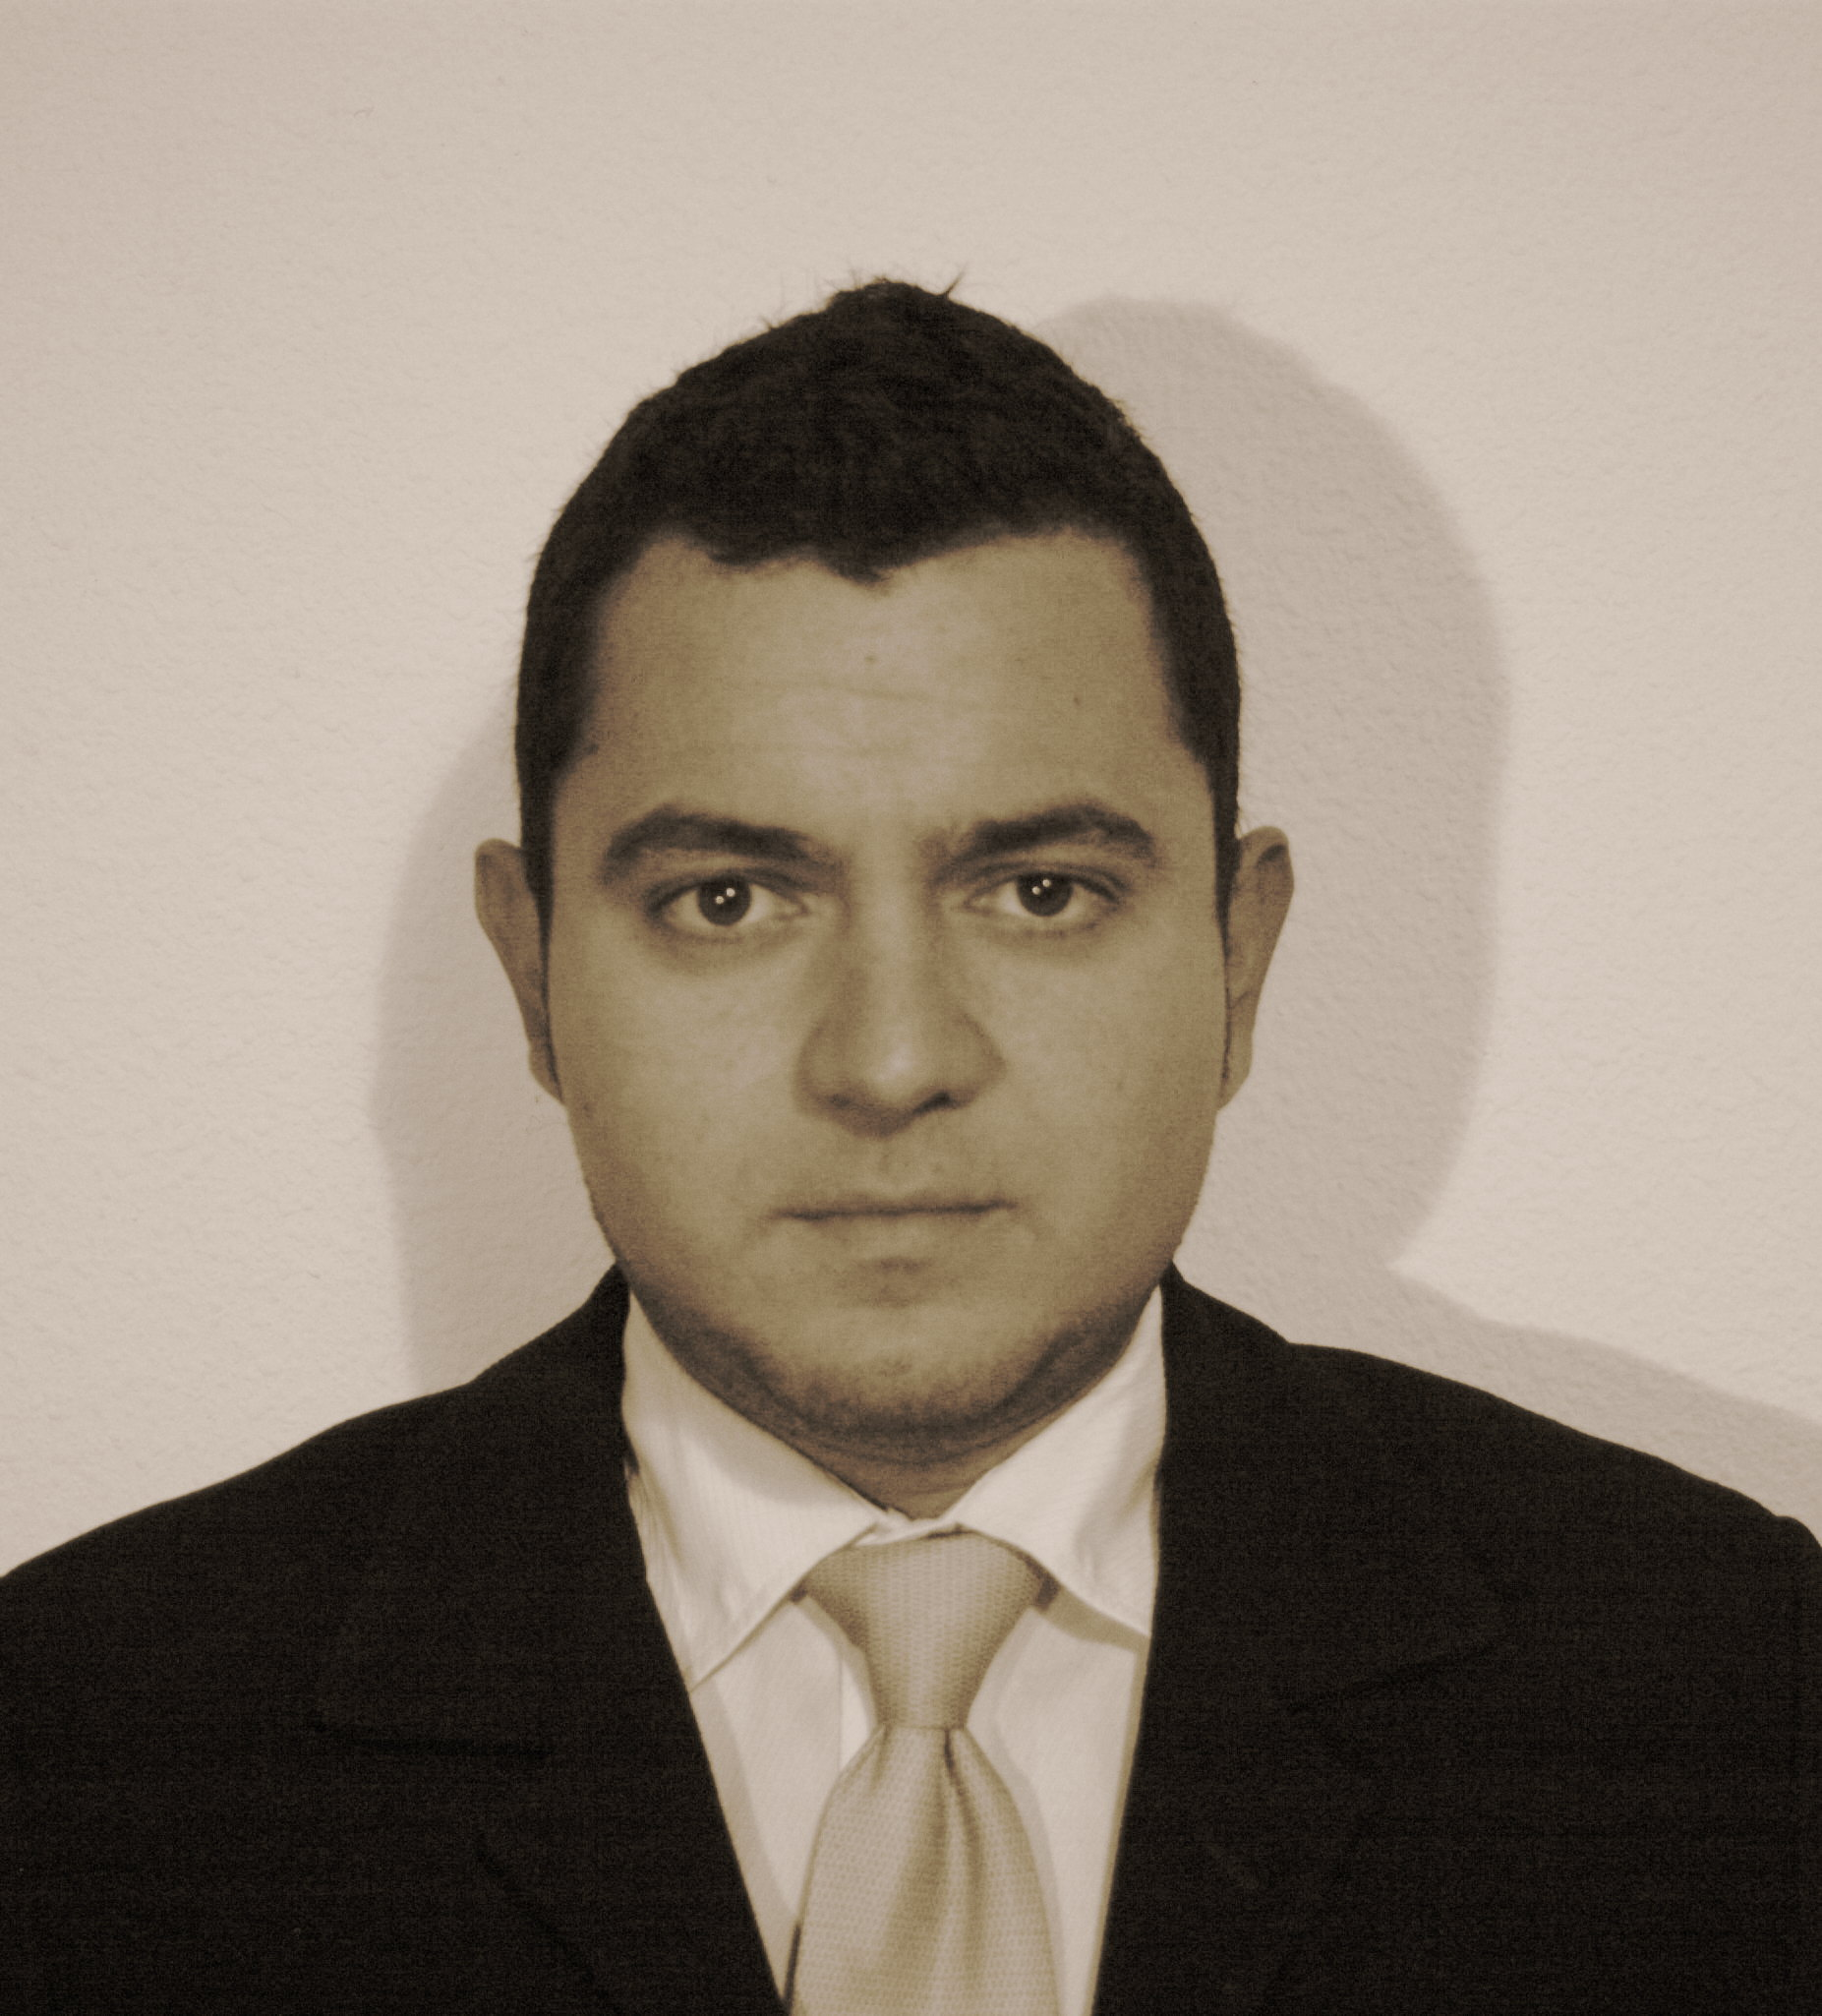
\includegraphics[scale=0.04]{CRW_8081-BW.jpeg}\\}  
\section{DATOS \\ PERSONALES\\}  
               %\textbf{Correo electr\'{o}nico:} \href{mailto:roberlamerma@gmail.com}{roberlamerma@gmail.com} \\
               
%               \begin{tabular}{>{\hfill}p{5cm}|p{11cm}}
%               & \textbf{Correo electr\'{o}nico:} \href{mailto:roberlamerma@gmail.com}{roberlamerma@gmail.com} \\
%               & \textbf{Direcci\'{o}n:} Calle Laforja, 8. pral-1era, 08006. Barcelona, Espa\~{n}a \\
%               & \textbf{Tel\'{e}fono:} 678714822 (m\'{o}vil) / 932178436 (domicilio)\\
%               & Carnet de Conducir\\
%               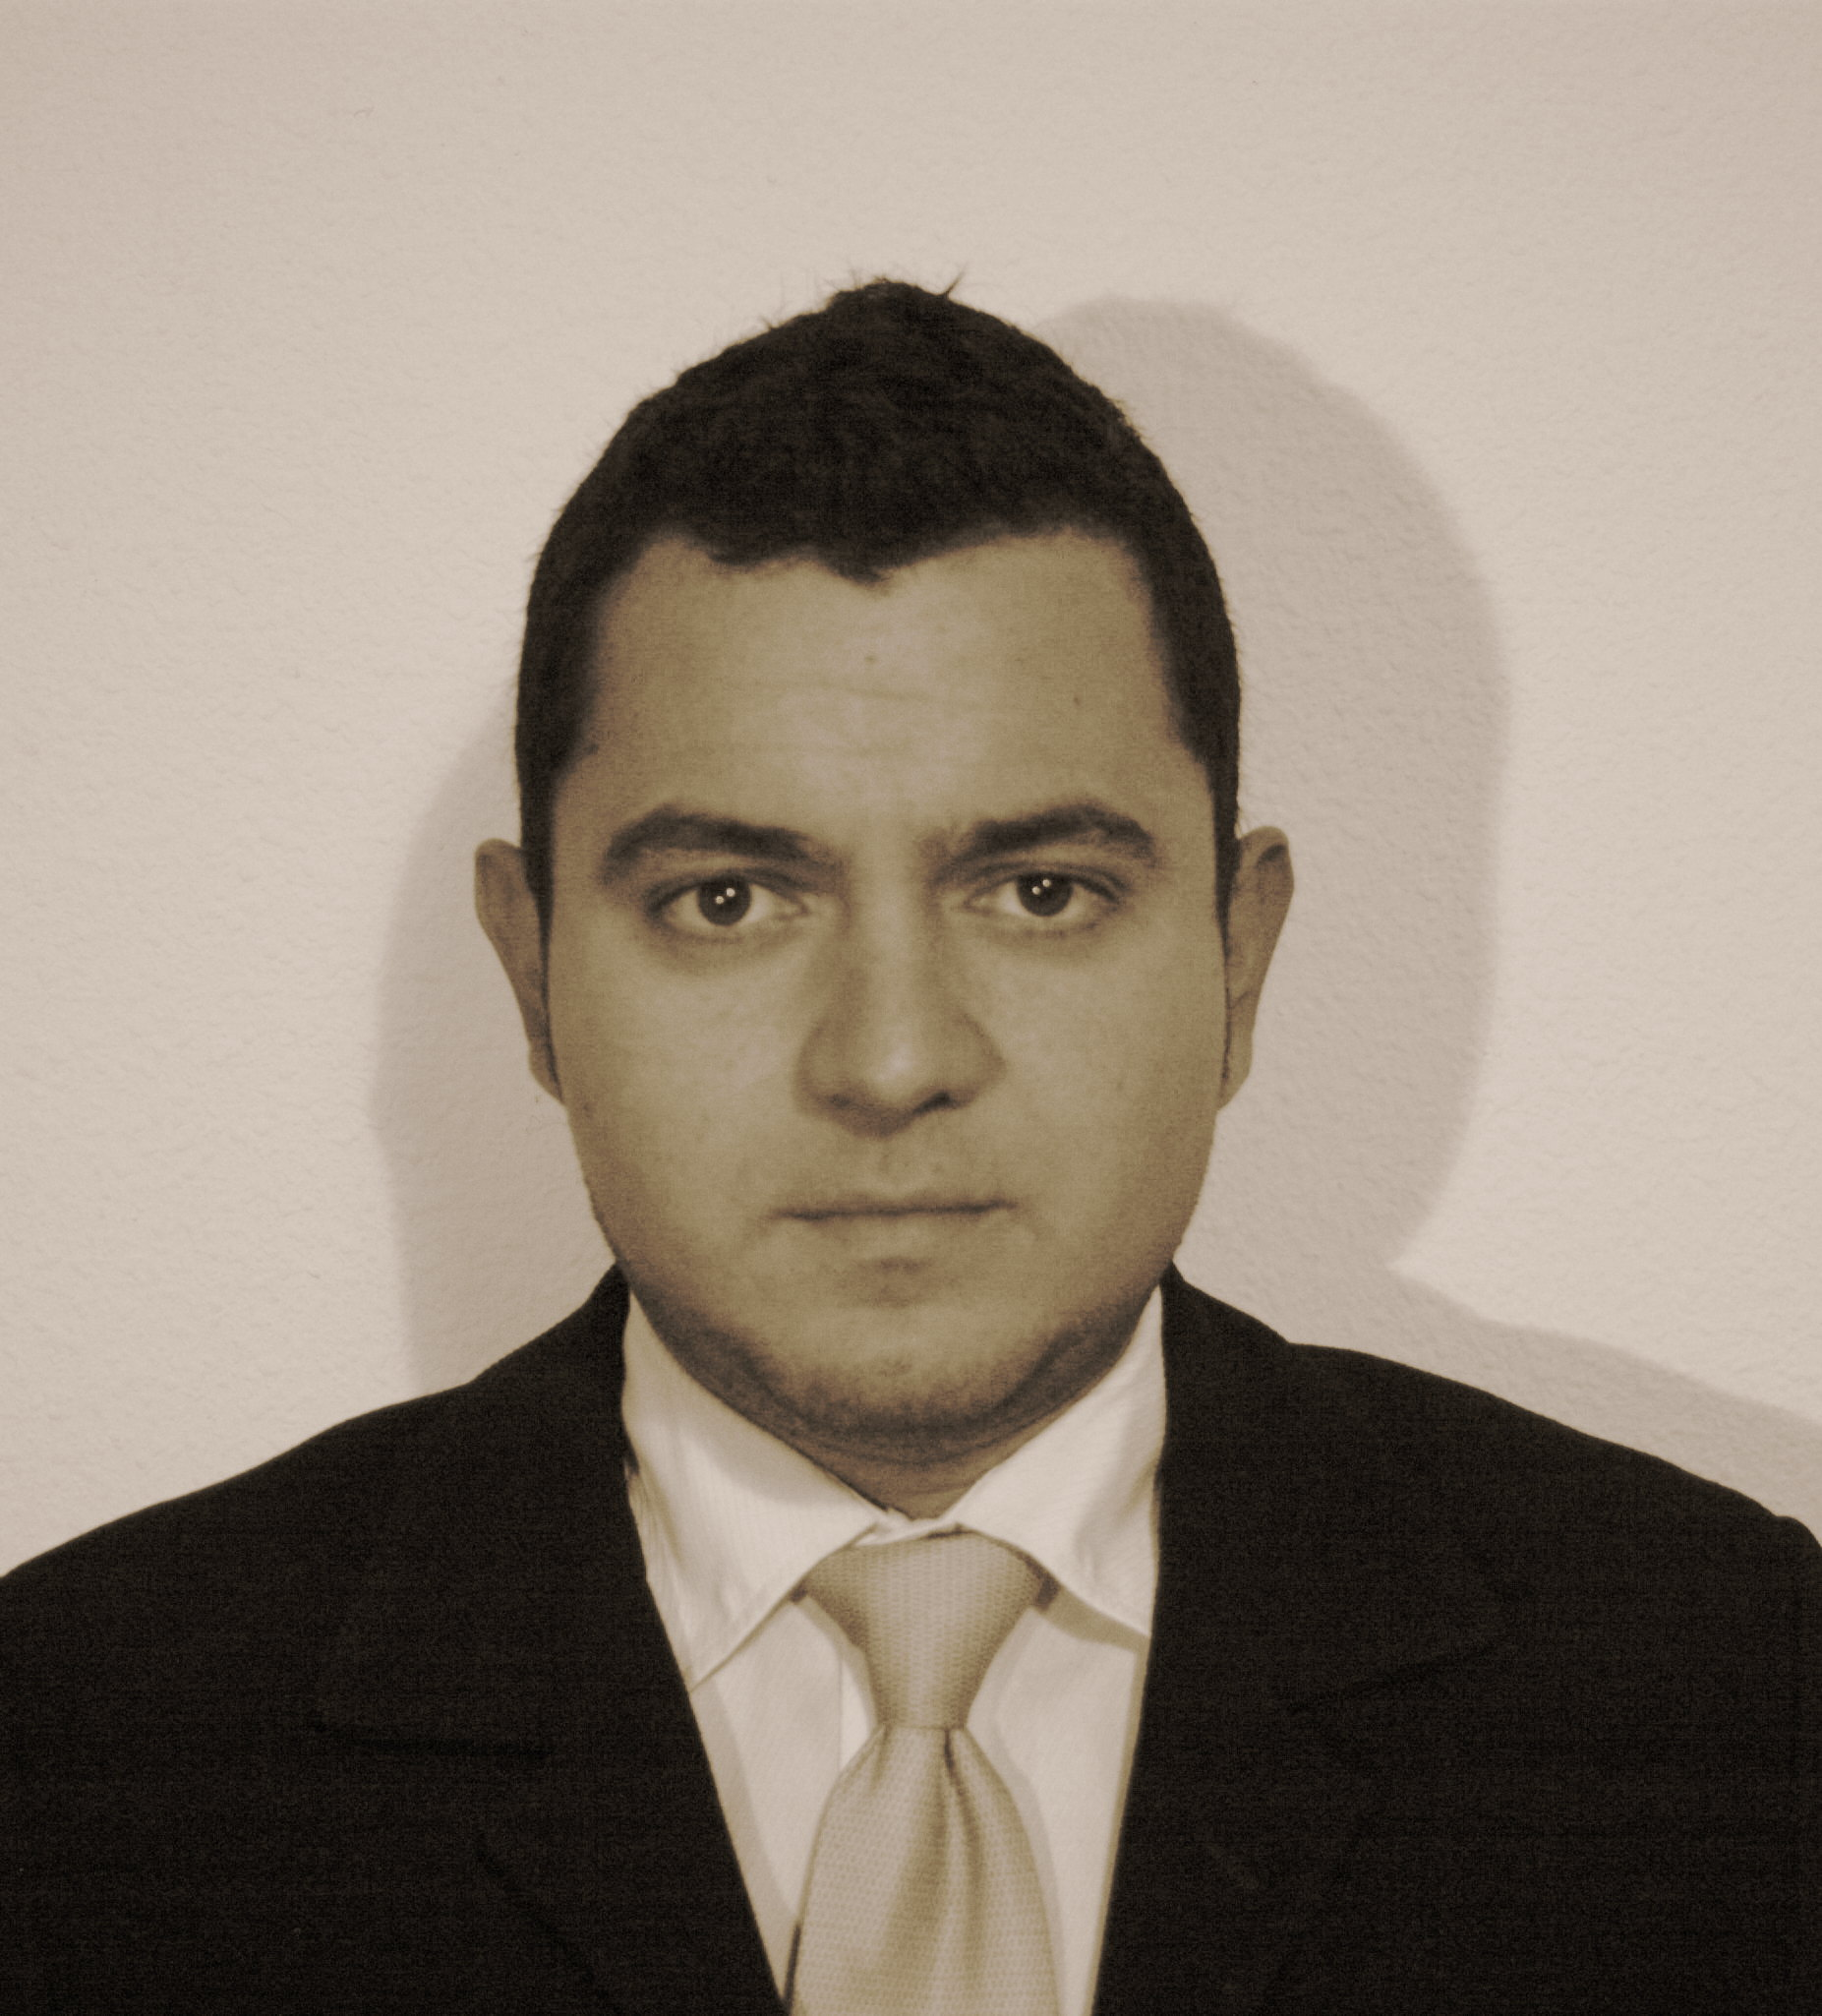
\includegraphics[scale=0.04]{CRW_8081-BW.jpeg} & Disponibilidad para viajar\\
%               \multicolumn{2}{c}{}
%               \end{tabular}

               % Sin foto...               
               \textbf{Correo electr\'{o}nico:} \href{mailto:roberlamerma@gmail.com}{roberlamerma@gmail.com} \\
               \textbf{Direcci\'{o}n:} Calle Londres 25, 6to-1era, 08029. Barcelona, Espa\~{n}a\\
               \textbf{Tel\'{e}fono:} 678714822 (m\'{o}vil)\\
               Carnet de Conducir y disponibilidad para viajar\\


\end{resume}
\end{document}







